\documentclass[a4paper, 12pt]{article}
% packages
\usepackage{amssymb}
\usepackage[fleqn]{mathtools}
\usepackage{tikz}
\usepackage{enumerate}
\usepackage{bussproofs}
\usepackage{xcolor}
\usepackage[margin=1.3cm]{geometry}
\usepackage{logicproof}
\usepackage{diagbox}
\usepackage{listings}
\usepackage{graphicx}
\usepackage{lstautogobble}
\usepackage{hyperref}
\usepackage{multirow}
\usepackage{tipa}
\usetikzlibrary{decorations.pathreplacing, arrows, shapes.gates.logic.US, circuits.logic.US, calc, automata, positioning}

% shorthand for verbatim
% this clashes with logicproof, so maybe fix this at some point?
\catcode`~=\active
\def~#1~{\texttt{#1}}

% code listing
\lstdefinestyle{main}{
    numberstyle=\tiny,
    breaklines=true,
    showspaces=false,
    showstringspaces=false,
    tabsize=2,
    numbers=left,
    basicstyle=\ttfamily,
    columns=fixed,
    fontadjust=true,
    basewidth=0.5em,
    autogobble,
    xleftmargin=3.0ex,
    mathescape=true
}
\newcommand{\dollar}{\mbox{\textdollar}} %
\lstset{style=main}

% augmented matrix
\makeatletter
\renewcommand*\env@matrix[1][*\c@MaxMatrixCols c]{%
\hskip -\arraycolsep
\let\@ifnextchar\new@ifnextchar
\array{#1}}
\makeatother

% ceiling / floor
\DeclarePairedDelimiter{\ceil}{\lceil}{\rceil}
\DeclarePairedDelimiter{\floor}{\lfloor}{\rfloor}

% custom commands
\newcommand{\indefint}[2]{\int #1 \, \mathrm{d}#2}
\newcommand{\defint}[4]{\int_{#1}^{#2} #3 \, \mathrm{d}#4}
\newcommand{\pdif}[2]{\frac{\partial #1}{\partial #2}}
\newcommand{\dif}[2]{\frac{\mathrm{d}#1}{\mathrm{d}#2}}
\newcommand{\limit}[2]{\raisebox{0.5ex}{\scalebox{0.8}{$\displaystyle{\lim_{#1 \to #2}}$}}}
\newcommand{\summation}[2]{\sum\limits_{#1}^{#2}}
\newcommand{\product}[2]{\prod\limits_{#1}^{#2}}
\newcommand{\intbracket}[3]{\left[#3\right]_{#1}^{#2}}
\newcommand{\ulsmash}[1]{\underline{\smash{#1}}}

\newcommand{\powerset}[0]{\wp}
\renewcommand{\emptyset}[0]{\varnothing}

\makeatletter
\newsavebox{\@brx}
\newcommand{\llangle}[1][]{\savebox{\@brx}{\(\m@th{#1\langle}\)}%
  \mathopen{\copy\@brx\kern-0.5\wd\@brx\usebox{\@brx}}}
\newcommand{\rrangle}[1][]{\savebox{\@brx}{\(\m@th{#1\rangle}\)}%
  \mathclose{\copy\@brx\kern-0.5\wd\@brx\usebox{\@brx}}}
\makeatother
\newcommand{\lla}{\llangle}
\newcommand{\rra}{\rrangle}
\newcommand{\la}{\langle}
\newcommand{\ra}{\rangle}
\newcommand{\crnr}[1]{\text{\textopencorner} #1 \text{\textcorner}}
\newcommand{\laplace}{\mathcal{L}}
\newcommand{\fourier}{\mathcal{F}}

\newcommand{\mat}[1]{\boldsymbol{#1}}
\renewcommand{\vec}[1]{\boldsymbol{#1}}
\newcommand{\rowt}[1]{\begin{bmatrix}
    #1
\end{bmatrix}^\top}

\newcommand{\unaryproof}[2]{\AxiomC{#1} \UnaryInfC{#2} \DisplayProof}
\newcommand{\binaryproof}[3]{\AxiomC{#1} \AxiomC{#2} \BinaryInfC{#3} \DisplayProof}
\newcommand{\trinaryproof}[4]{\AxiomC{#1} \AxiomC{#2} \AxiomC{#3} \TrinaryInfC{#4} \DisplayProof}

\newcommand{\axiom}[1]{\AxiomC{#1}}
\newcommand{\unary}[1]{\UnaryInfC{#1}}
\newcommand{\binary}[1]{\BinaryInfC{#1}}
\newcommand{\trinary}[1]{\TrinaryInfC{#1}}
\newcommand{\quaternary}[1]{\QuaternaryInfC{#1}}
\newcommand{\quinary}[1]{\QuinaryInfC{#1}}
\newcommand{\dproof}[0]{\DisplayProof}

\newcommand{\bnfsep}[0]{\ |\ }
\newcommand{\concsep}[0]{\ ||\ }
\newcommand{\ttbs}{\char`\\}

\newcommand{\violet}[1]{\textcolor{violet}{#1}}
\newcommand{\blue}[1]{\textcolor{blue}{#1}}
\newcommand{\red}[1]{\textcolor{red}{#1}}

% no indent
\setlength\parindent{0pt}

% reasoning proofs
\usepackage{ltablex}
\usepackage{environ}
\keepXColumns
\NewEnviron{reasoning}{
    \begin{tabularx}{\textwidth}{rlX}
        \BODY
    \end{tabularx}
}
\newcommand{\proofline}[3]{$(#1)$ & $#2$ & \hfill #3 \smallskip \\}
\newcommand{\proofarbitrary}[1]{& take arbitrary $#1$ \smallskip \\}
\newcommand{\prooftext}[1]{\multicolumn{3}{l}{#1} \smallskip \\}
\newcommand{\proofmath}[3]{$#1$ & = $#2$ & \hfill #3 \smallskip \\}
\newcommand{\prooftherefore}[1]{& $\therefore #1$ \smallskip \\}
\newcommand{\proofbc}[0]{\prooftext{\textbf{Base Case}}}
\newcommand{\proofis}[0]{\prooftext{\textbf{Inductive Step}}}

% reasoning er diagrams
\newcommand{\nattribute}[4]{
    \node[draw, state, inner sep=0cm, minimum size=0.2cm, label=#3:{#4}] (#1) at (#2) {};
}
\newcommand{\mattribute}[4]{
    \node[draw, state, accepting, inner sep=0cm, minimum size=0.2cm, label=#3:{#4}] (#1) at (#2) {};
}
\newcommand{\dattribute}[4]{
    \node[draw, state, dashed, inner sep=0cm, minimum size=0.2cm, label=#3:{#4}] (#1) at (#2) {};
}
\newcommand{\entity}[3]{
    \node[] (#1-c) at (#2) {#3};
    \node[inner sep=0cm] (#1-l) at ($(#1-c) + (-1, 0)$) {};
    \node[inner sep=0cm] (#1-r) at ($(#1-c) + (1, 0)$) {};
    \node[inner sep=0cm] (#1-u) at ($(#1-c) + (0, 0.5)$) {};
    \node[inner sep=0cm] (#1-d) at ($(#1-c) + (0, -0.5)$) {};
    \draw
    ($(#1-c) + (-1, 0.5)$) -- ($(#1-c) + (1, 0.5)$) -- ($(#1-c) + (1, -0.5)$) -- ($(#1-c) + (-1, -0.5)$) -- cycle;
}
\newcommand{\relationship}[3]{
    \node[] (#1-c) at (#2) {#3};
    \node[inner sep=0cm] (#1-l) at ($(#1-c) + (-1, 0)$) {};
    \node[inner sep=0cm] (#1-r) at ($(#1-c) + (1, 0)$) {};
    \node[inner sep=0cm] (#1-u) at ($(#1-c) + (0, 1)$) {};
    \node[inner sep=0cm] (#1-d) at ($(#1-c) + (0, -1)$) {};
    \draw
    ($(#1-c) + (-1, 0)$) -- ($(#1-c) + (0, 1)$) -- ($(#1-c) + (1, 0)$) -- ($(#1-c) + (0, -1)$) -- cycle;
}

% actual document
\begin{document}
    \section*{CO221 - Compilers}
        \subsection*{6th January 2020}
            A compiler is a program which processes programs, including translating a program written in one language (usually higher level) to another programming language (usually in a lower level).
            In our course, the focus is to generate assembly code from the high level language.
            This translation goes between high level human concepts, and the data manipulation the machine performs.
            \subsubsection*{Structure}
                The general structure of a compiler is as follows;
                \begin{enumerate}[1.]
                    \itemsep0em
                    \item \textbf{input} \hfill takes in an input program in some language
                    \item \textbf{analysis} \hfill constructs an internal representation of the source structure
                    \item \textbf{synthesis} \hfill walks the representation to generate the output code
                    \item \textbf{output} \hfill creates an output in the target language
                \end{enumerate}
                In more detail, it can be represented as follows;
                \begin{center}
                    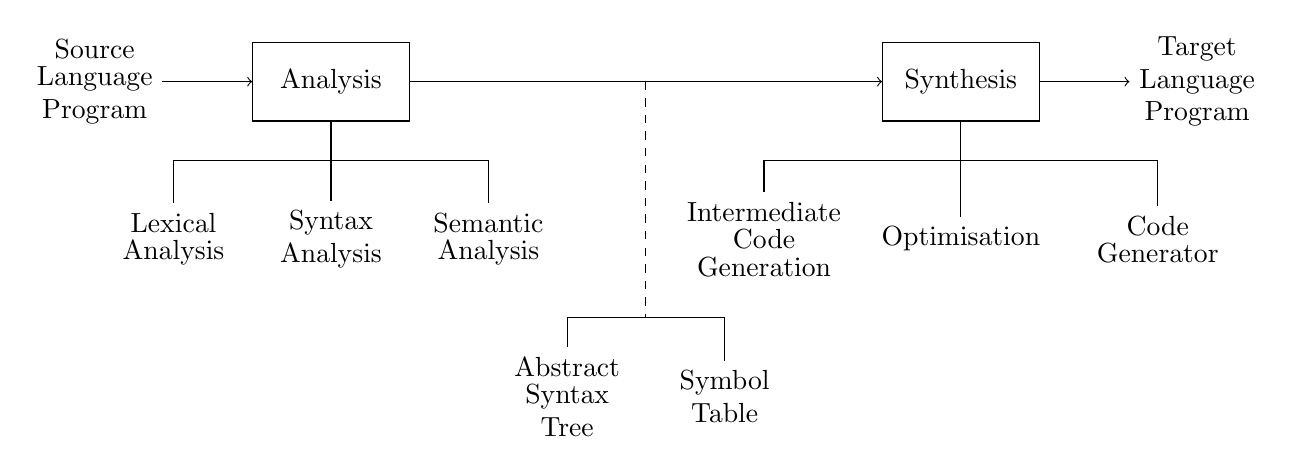
\begin{tikzpicture}
                        \node (slp) at (0, 0) {\shortstack{Source \\ Language \\ Program}};
                        \node (a) at (3, 0) {Analysis};
                        \node (s) at (11, 0) {Synthesis};
                        \node (tlp) at (14, 0) {\shortstack{Target \\ Language \\ Program}};

                        \node (la) at (1, -2) {\shortstack{Lexical \\ Analysis}};
                        \node (sa1) at (3, -2) {\shortstack{Syntax \\ Analysis}};
                        \node (sa2) at (5, -2) {\shortstack{Semantic \\ Analysis}};

                        \node (icg) at (8.5, -2) {\shortstack{Intermediate \\ Code \\ Generation}};
                        \node (o) at (11, -2) {Optimisation};
                        \node (cg) at (13.5, -2) {\shortstack{Code \\ Generator}};

                        \node (ast) at (6, -4) {\shortstack{Abstract \\ Syntax \\ Tree}};
                        \node (st) at (8, -4) {\shortstack{Symbol \\ Table}};

                        \draw
                        (slp) edge[->] (2, 0)
                        (4, 0) edge[->] (10, 0)
                        (12, 0) edge[->] (tlp)

                        (3, -0.5) -- (3, -1)
                        (11, -0.5) -- (11, -1)
                        (7, 0) edge[dashed] (7, -3)

                        (1, -1) -- (5, -1)
                        (1, -1) -- (la)
                        (3, -1) -- (sa1)
                        (5, -1) -- (sa2)

                        (8.5, -1) -- (13.5, -1)
                        (8.5, -1) -- (icg)
                        (11, -1) -- (o)
                        (13.5, -1) -- (cg)

                        (6, -3) -- (8, -3)
                        (6, -3) -- (ast)
                        (8, -3) -- (st)

                        (2, 0.5) -- (4, 0.5) -- (4, -0.5) -- (2, -0.5) -- cycle
                        (10, 0.5) -- (12, 0.5) -- (12, -0.5) -- (10, -0.5) -- cycle;
                    \end{tikzpicture}
                \end{center}
                \begin{itemize}
                    \itemsep0em
                    \item \textbf{lexical analysis} looks at characters of input program, analyses which are keywords (such as converting ~if~, and ~while~ to corresponding tokens), which are user defined words, and which are punctuation, etc.
                    \item \textbf{syntax analysis} discovers structure of input
                    \item \textbf{semantic analysis} checks that variables are declared before they are used, and that they are used consistently with their types etc.
                \end{itemize}
                Simple compilers go straight to code generation, but optimising compilers do several passes of intermediate code generation and optimisation.
                \smallskip

                The symbol table holds data on variables, such as types.
                Sometimes we need to know the type of the variable, in order to generate code for the variable, for example if we were to print a variable, it would need to generate different code for strings than it would need to do for integers.
                Scope rules are also needed.
            \subsubsection*{Phases}
                Whether all of these phases are done in the order shown is a design choice.
                For example, lexical analysis and syntax analysis are often interleaved.
                This can be done when the syntax analysis stage needs the next symbol, and therefore the lexical analysis stage can be used.
                \begin{center}
                    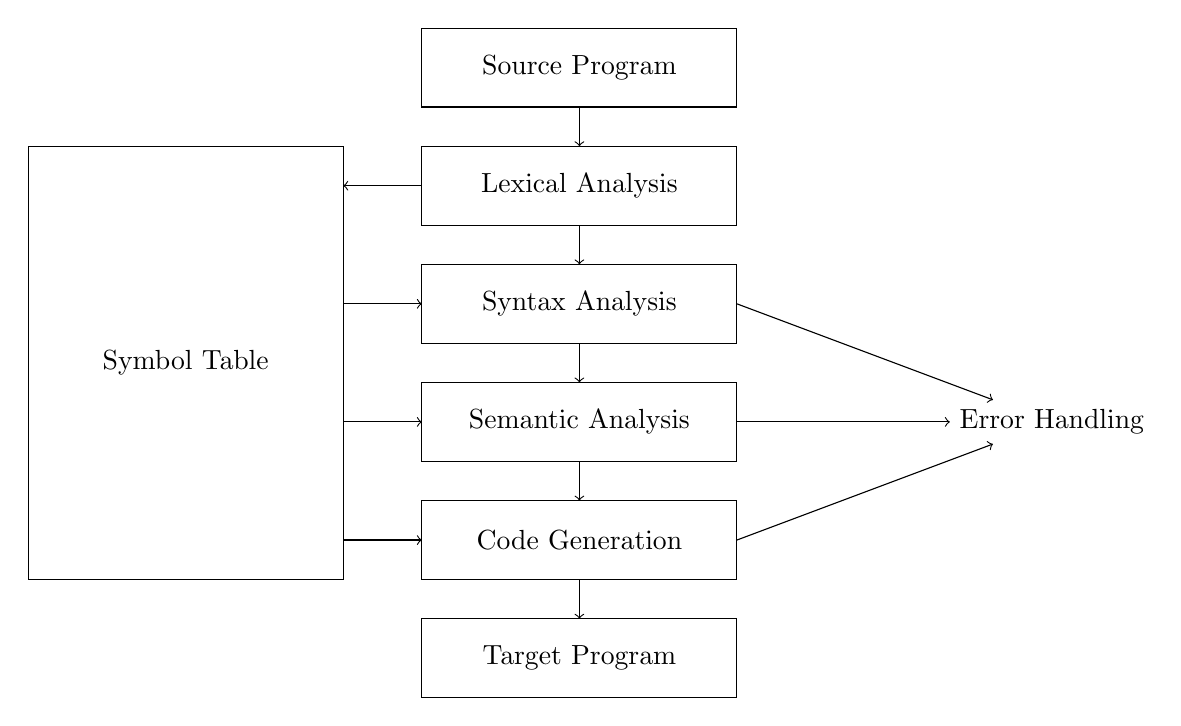
\begin{tikzpicture}
                        \node () at (0, 0) {Source Program};
                        \node () at (0, -1.5) {Lexical Analysis};
                        \node () at (0, -3) {Syntax Analysis};
                        \node () at (0, -4.5) {Semantic Analysis};
                        \node () at (0, -6) {Code Generation};
                        \node () at (0, -7.5) {Target Program};
                        \node () at (-5, -3.75) {Symbol Table};
                        \node (eh) at (6, -4.5) {Error Handling};

                        \draw
                        (-2, 0.5) -- (2, 0.5) -- (2, -0.5) -- (-2, -0.5) -- cycle
                        (-2, -1) -- (2, -1) -- (2, -2) -- (-2, -2) -- cycle
                        (-2, -2.5) -- (2, -2.5) -- (2, -3.5) -- (-2, -3.5) -- cycle
                        (-2, -4) -- (2, -4) -- (2, -5) -- (-2, -5) -- cycle
                        (-2, -5.5) -- (2, -5.5) -- (2, -6.5) -- (-2, -6.5) -- cycle
                        (-2, -7) -- (2, -7) -- (2, -8) -- (-2, -8) -- cycle
                        (-7, -1) -- (-3, -1) -- (-3, -6.5) -- (-7, -6.5) -- cycle

                        (0, -0.5) edge[->] (0, -1)
                        (0, -2) edge[->] (0, -2.5)
                        (0, -3.5) edge[->] (0, -4)
                        (0, -5) edge[->] (0, -5.5)
                        (0, -6.5) edge[->] (0, -7)
                        (-2, -1.5) edge[->] (-3, -1.5)
                        (-3, -3) edge[->] (-2, -3)
                        (2, -3) edge[->] (eh)
                        (-3, -4.5) edge[->] (-2, -4.5)
                        (2, -4.5) edge[->] (eh)
                        (-3, -6) edge[->] (-2, -6)
                        (2, -6) edge[->] (eh);
                    \end{tikzpicture}
                \end{center}
            \subsubsection*{Syntax Analysis}
                This is also known as parsing.
                Languages have a grammatical structure specified by grammatical rules in a \textbf{context-free grammar} such as BNF (\textbf{Backus-Naur Form}).
                The output of the analyser is a data structure which represents the program structure; an \textbf{abstract syntax tree}.
                The writer of the compiler must design the AST carefully such that it is easy to build, as well as easy to use by the code generator.
                \smallskip

                A language specification consists of the following;
                \begin{itemize}
                    \itemsep0em
                    \item \textbf{syntax} \hfill grammatical structure
                        \subitem in order to determine that a program is syntactically correct, one must determine how the rules were used to construct it
                    \item \textbf{semantics} \hfill meaning
                \end{itemize}
                For example, we can encode the rules for a statement as follows (anything in quotes is a terminal), in BNF;
                \begin{center}
                    stat $\to$ 'if' '(' exp ')' stat 'else' stat
                \end{center}
                Each BNF production is a valid way for a non-terminal (LHS) to be expanded (RHS) into a combination of terminals and non-terminals.
                Only terminals can appear in the final results (they are lexical tokens).
                \smallskip

                To prove the following is a valid example of stat, we'd need to show that a can be derived from exp, and that both b and c can be derived from stat.
                \begin{center}
                    if ( a ) b else c
                \end{center}
            \subsubsection*{Context-Free Grammars}
                Formally, a context-free grammar consists of the following four components;
                \begin{itemize}
                    \itemsep0em
                    \item $S$ \hfill a non-terminal start symbol
                    \item $P$ \hfill a set of productions
                    \item $t$ \hfill a set of tokens (terminals)
                    \item $nt$ \hfill a set of non-terminals
                \end{itemize}
                For example, consider the following BNF, and their associated components;
                \begin{align*}
                    \text{bin} \to &\ \text{bin '+' dig} \bnfsep \text{bin '-' dig} \bnfsep \text{dig} \\
                    \text{dig} \to &\ \text{'0'} \bnfsep \text{'1'} \\
                    t = &\ \{ \text{'+'}, \text{'-'}, \text{'0'}, \text{'1'}\} \\
                    nt = &\ \{ \text{bin}, \text{dig}\} \\
                    S = &\ \text{bin}
                \end{align*}
                A string of only terminals (\textbf{sentential form}) can be derived using the grammar by beginning with the start symbol, and repeatedly replacing each non-terminal with the RHS from a corresponding production.
                We refer to the set of all sentential forms derived from the start symbol as the \textbf{language} of a grammar.
                \smallskip

                We can prove that some string is in the language of a grammar by constructing a \textbf{parse tree}.
                For example, to prove that $\text{"1+1-0"} \in L(G)$, and $\text{"1+1"} \in L(G)$ we can use the following trees;
                \begin{center}
                    \begin{tikzpicture}[x=2cm]
                        \node (b1) at (0, 0) {bin};
                        \node (b2) at (-1, -1) {bin};
                        \node (b3) at (-2, -2) {bin};
                        \node (d1) at (1, -1) {dig};
                        \node (d2) at (0, -2) {dig};
                        \node (d3) at (-2, -3) {dig};
                        \node (o1) at (-2, -4) {'1'};
                        \node (o2) at (0, -3) {'1'};
                        \node (z) at (1, -2) {'0'};
                        \node (m) at (0, -1) {'-'};
                        \node (p) at (-1, -2) {'+'};

                        \draw
                        (b1) -- (d1) -- (z)
                        (b1) -- (m)
                        (b2) -- (d2) -- (o2)
                        (b2) -- (p)
                        (b1) -- (b2) -- (b3) -- (d3) -- (o1);
                    \end{tikzpicture}
                    \hfill
                    \begin{tikzpicture}[x=2cm]
                        \node (b1) at (0, 0) {bin};
                        \node (b2) at (-1, -1) {bin};
                        \node (d1) at (1, -1) {dig};
                        \node (d2) at (-1, -2) {dig};
                        \node (o1) at (-1, -3) {'1'};
                        \node (o2) at (1, -2) {'1'};
                        \node (p) at (0, -1) {'+'};

                        \draw
                        (b1) -- (d1) -- (o2)
                        (b1) -- (p)
                        (b1) -- (b2) -- (d2) -- (o1);
                    \end{tikzpicture}
                \end{center}
            \subsubsection*{Ambiguity}
                A grammar is referred to as \textbf{ambiguous} if its language contains strings which can be generated in two different ways.
                Essentially, there exists some string in $L(G)$ which has two different parse trees.
                Consider string "1 + a - 3" in the following grammar, and the parse tree(s) associated;
                \begin{center}
                    exp $\to$ exp '+' exp \vline\ exp '-' exp \vline\ const \vline\ ident
                \end{center}
                \begin{center}
                    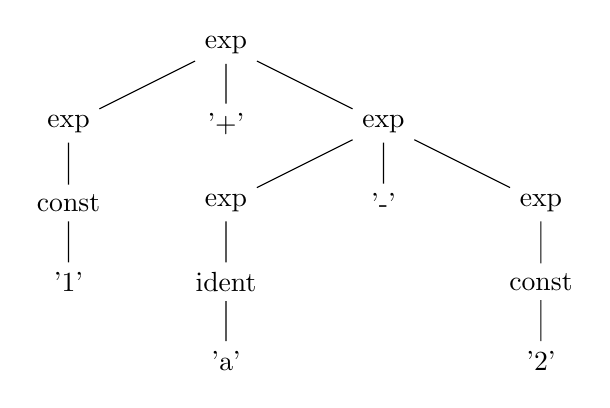
\begin{tikzpicture}[x=2cm]
                        \node (e1) at (0, 0) {exp};
                        \node (e2) at (-1, -1) {exp};
                        \node (e3) at (1, -1) {exp};
                        \node (e4) at (0, -2) {exp};
                        \node (e5) at (2, -2) {exp};
                        \node (c1) at (-1, -2) {const};
                        \node (c2) at (2, -3) {const};
                        \node (i) at (0, -3) {ident};
                        \node (p) at (0, -1) {'+'};
                        \node (m) at (1, -2) {'-'};
                        \node (o) at (-1, -3) {'1'};
                        \node (a) at (0, -4) {'a'};
                        \node (t) at (2, -4) {'2'};
                        \draw
                        (e1) -- (e2) -- (c1) -- (o)
                        (e1) -- (p)
                        (e1) -- (e3) -- (e4) -- (i) -- (a)
                        (e3) -- (m)
                        (e3) -- (e5) -- (c2) -- (t);
                    \end{tikzpicture}
                    \hfill
                    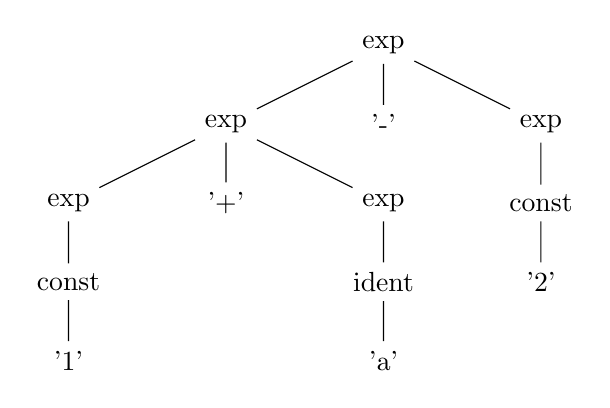
\begin{tikzpicture}[x=2cm]
                        \node (e1) at (0, 0) {exp};
                        \node (e2) at (-1, -1) {exp};
                        \node (e3) at (1, -1) {exp};
                        \node (e4) at (-2, -2) {exp};
                        \node (e5) at (0, -2) {exp};
                        \node (c1) at (1, -2) {const};
                        \node (c2) at (-2, -3) {const};
                        \node (i) at (0, -3) {ident};
                        \node (p) at (-1, -2) {'+'};
                        \node (m) at (0, -1) {'-'};
                        \node (o) at (-2, -4) {'1'};
                        \node (a) at (0, -4) {'a'};
                        \node (t) at (1, -3) {'2'};
                        \draw
                        (e1) -- (e2) -- (e4) -- (c2) -- (o)
                        (e1) -- (m)
                        (e1) -- (e3) -- (c1) -- (t)
                        (e2) -- (p)
                        (e2) -- (e5) -- (i) -- (a);
                    \end{tikzpicture}
                \end{center}
                While the string is still valid, and in the language, our issue is with the ambiguity, as we want to generate a program uniquely.
                The reason our grammar is broken is due to the recursive use of the non-terminal exp on both sides, which means we're given a choice of which side to expand when generating.
            \subsubsection*{Associativity and Precedence}
                For our example language, we're using all left-associative operators.
                We also want to maintain that '*' and '/' have higher precedence than '+' and '-'.
                One way of doing this is to split the grammar into layers, by having separate non-terminals for precedence levels.
                This method can be done with the following unambiguous grammar for arithmetic expressions;
                \begin{align*}
                    \text{exp} & \to \text{exp '+' term} \bnfsep \text{exp '-' term} \bnfsep \text{term} \\
                    \text{term} & \to \text{term '*' factor} \bnfsep \text{term '/' factor} \bnfsep \text{factor} \\
                    \text{factor} & \to \text{const} \bnfsep \text{ident}
                \end{align*}
                Now, we can unambiguously generate the parse tree (and thus the unique abstract syntax tree) for "9+5*2";
                \begin{center}
                    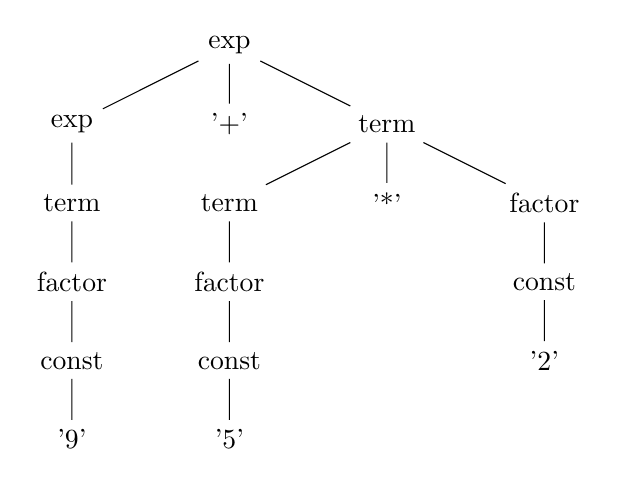
\begin{tikzpicture}[x=2cm]
                        \node (e1) at (0, 0) {exp};
                        \node (e2) at (-1, -1) {exp};
                        \node (t1) at (1, -1) {term};
                        \node (t2) at (-1, -2) {term};
                        \node (t3) at (0, -2) {term};
                        \node (f1) at (2, -2) {factor};
                        \node (f2) at (-1, -3) {factor};
                        \node (f3) at (0, -3) {factor};
                        \node (c1) at (2, -3) {const};
                        \node (c2) at (-1, -4) {const};
                        \node (c3) at (0, -4) {const};
                        \node (p) at (0, -1) {'+'};
                        \node (m) at (1, -2) {'*'};
                        \node (n) at (-1, -5) {'9'};
                        \node (f) at (0, -5) {'5'};
                        \node (t) at (2, -4) {'2'};
                        \draw
                        (e1) -- (e2) -- (t2) -- (f2) -- (c2) -- (n)
                        (e1) -- (p)
                        (e1) -- (t1) -- (t3) -- (f3) -- (c3) -- (f)
                        (t1) -- (m)
                        (t1) -- (f1) -- (c1) -- (t);
                    \end{tikzpicture}
                    \hfill
                    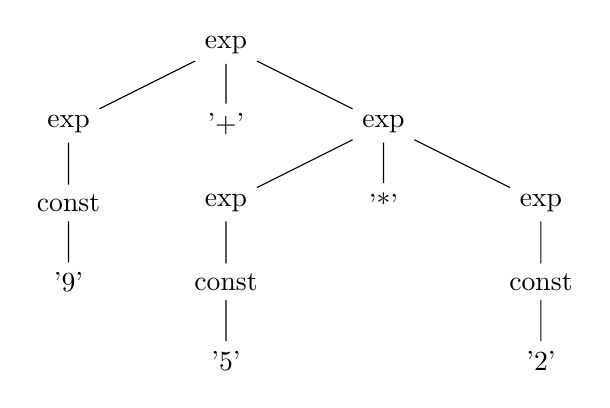
\begin{tikzpicture}[x=2cm]
                        \node (e1) at (0, 0) {exp};
                        \node (e2) at (-1, -1) {exp};
                        \node (p) at (0, -1) {'+'};
                        \node (e3) at (1, -1) {exp};
                        \node (c1) at (-1, -2) {const};
                        \node (e4) at (0, -2) {exp};
                        \node (m) at (1, -2) {'*'};
                        \node (e5) at (2, -2) {exp};
                        \node (n) at (-1, -3) {'9'};
                        \node (c2) at (0, -3) {const};
                        \node (c3) at (2, -3) {const};
                        \node (f) at (0, -4) {'5'};
                        \node (t) at (2, -4) {'2'};
                        \draw
                        (e1) -- (e2) -- (c1) -- (n)
                        (e1) -- (p)
                        (e1) -- (e3) -- (e4) -- (c2) -- (f)
                        (e3) -- (m)
                        (e3) -- (e5) -- (c3) -- (t);
                    \end{tikzpicture}
                \end{center}
                It's important to note that the \textbf{abstract} syntax tree doesn't need this in contrast, as only the parse tree needs it.
            \subsubsection*{Parsers}
                The parser checks that the input is grammatically correct, and builds an AST representing the structure.
                In general, there are two classes of parsing algorithms;
                \begin{itemize}
                    \itemsep0em
                    \item \textbf{top-down / predictive} \hfill we are using recursive descent
                    \item \textbf{bottom-up} \hfill also known as shift-reduce
                \end{itemize}
                For this, we will use the input "~begin S; S; end~", with the following grammar;
                \begin{align*}
                    \text{stat} & \to ~'begin'~\ \text{statlist} \bnfsep ~'S'~ \\
                    \text{statlist} & \to ~'end'~ \bnfsep \text{stat}\ ~';'~\ \text{statlist}
                \end{align*}
                When we start top-down parsing, we start with the non-terminal stat.
                The first token we identify is the ~'begin'~, thus our tree becomes the following;
                \begin{center}
                    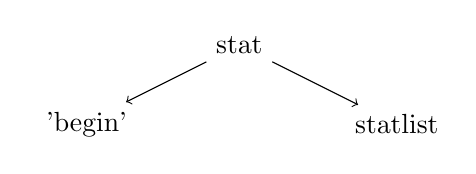
\begin{tikzpicture}[x=2cm]
                        \node (s) at (0, 0) {stat};
                        \node (b) at (-1, -1) {~'begin'~};
                        \node (sl) at (1, -1) {statlist};

                        \draw
                        (s) edge[->] (b)
                        (s) edge[->] (sl);
                    \end{tikzpicture}
                \end{center}
                However, as the next symbol isn't the terminal ~'end'~, we have to use an alternative.
                As we only have one alternative, we can predict it, and thus the tree becomes;
                \begin{center}
                    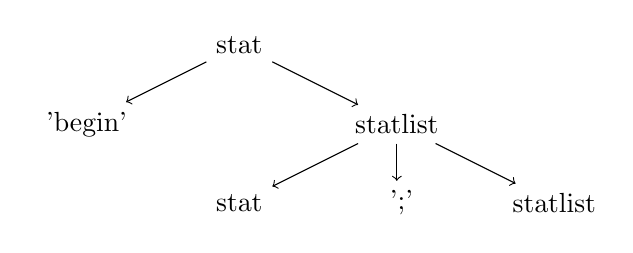
\begin{tikzpicture}[x=2cm]
                        \node (s) at (0, 0) {stat};
                        \node (b) at (-1, -1) {~'begin'~};
                        \node (sl) at (1, -1) {statlist};
                        \node (s2) at (0, -2) {stat};
                        \node (sc) at (1, -2) {~';'~};
                        \node (sl2) at (2, -2) {statlist};

                        \draw
                        (s) edge[->] (b)
                        (s) edge[->] (sl)
                        (sl) edge[->] (s2)
                        (sl) edge[->] (sc)
                        (sl) edge[->] (sl2);
                    \end{tikzpicture}
                \end{center}
                As the next symbols are the terminal ~'S'~, and the terminal ~';'~, we can tick them off, thus the tree becomes;
                \begin{center}
                    \begin{tikzpicture}[x=2cm]
                        \node (s) at (0, 0) {stat};
                        \node (b) at (-1, -1) {~'begin'~};
                        \node (sl) at (1, -1) {statlist};
                        \node (s2) at (0, -2) {stat};
                        \node (sc) at (1, -2) {~';'~};
                        \node (sl2) at (2, -2) {statlist};
                        \node (st) at (0, -3) {~'S'~};

                        \draw
                        (s) edge[->] (b)
                        (s) edge[->] (sl)
                        (sl) edge[->] (s2)
                        (sl) edge[->] (sc)
                        (sl) edge[->] (sl2)
                        (s2) edge[->] (st);
                    \end{tikzpicture}
                \end{center}
                This process continues, until we reach the final tree;
                \begin{center}
                    \begin{tikzpicture}[x=2cm]
                        \node (s) at (0, 0) {stat};
                        \node (b) at (-1, -1) {~'begin'~};
                        \node (sl) at (1, -1) {statlist};
                        \node (s2) at (0, -2) {stat};
                        \node (sc) at (1, -2) {~';'~};
                        \node (sl2) at (2, -2) {statlist};
                        \node (st) at (0, -3) {~'S'~};
                        \node (s3) at (1, -3) {stat};
                        \node (sc2) at (2, -3) {~';'~};
                        \node (sl3) at (3, -3) {statlist};
                        \node (st2) at (1, -4) {~'S'~};
                        \node (e) at (3, -4) {~'end'~};

                        \draw
                        (s) edge[->] (b)
                        (s) edge[->] (sl)
                        (sl) edge[->] (s2)
                        (sl) edge[->] (sc)
                        (sl) edge[->] (sl2)
                        (s2) edge[->] (st)
                        (sl2) edge[->] (s3)
                        (sl2) edge[->] (sc2)
                        (sl2) edge[->] (sl3)
                        (s3) edge[->] (st2)
                        (sl3) edge[->] (e);
                    \end{tikzpicture}
                \end{center}
                On the other hand, bottom-up parsing tries to use all the RHSs (whereas top-down tries to match a non-terminal by trying each of the RHSs), and replaces it with a non-terminal, by using the production in reverse.
                Bottom-up succeeds when the whole input is replaced by the start symbol.
                \smallskip

                In general, we push the current symbol onto the stack (or the reduction if we can reduce it).
                For example, once we encounter ~'S'~, we can reduce it to stat, and similarly once we encounter ~'end'~, we can reduce it to statlist.
                \begin{center}
                    \begin{tabular}{|r|c|l|l|l|}
                        \hline
                        stack & current symbol & remaining tokens & S/R & note \\
                        \hline
                        & ~'begin'~ & ~'S'~ ~';'~ ~'S'~ ~';'~ ~'end'~ & S & nothing to do yet \\
                        ~'begin'~ & \violet{~'S'~} & ~';'~ ~'S'~ ~';'~ ~'end'~ & R & terminal for stat \\
                        ~'begin'~ & \blue{stat} & ~';'~ ~'S'~ ~';'~ ~'end'~ & S & no more work \\
                        ~'begin'~ \blue{stat} & ~';'~ & ~'S'~ ~';'~ ~'end'~ & S & nothing to do yet \\
                        ~'begin'~ \blue{stat} ~';'~ & \violet{~'S'~} & ~';'~ ~'end'~ & R & terminal for stat \\
                        ~'begin'~ stat ~';'~ & \blue{stat} & ~';'~ ~'end'~ & S & no more work \\
                        ~'begin'~ stat ~';'~ \blue{stat} & ~';'~ & ~'end'~ & S & nothing to do yet \\
                        ~'begin'~ stat ~';'~ stat ~';'~ & \violet{~'end'~} & & R & terminal for statlist \\
                        ~'begin'~ stat ~';'~ stat ~';'~ & \blue{statlist} & & & \\
                        ~'begin'~ stat ~';'~ \violet{stat} \violet{~';'~} & \violet{statlist} & & R & match for statlist \\
                        ~'begin'~ stat ~';'~ & \blue{statlist} & & & \\
                        ~'begin'~ \violet{stat} \violet{~';'~} & \violet{statlist} & & R & match for statlist \\
                        ~'begin'~ & \blue{statlist} & & & \\
                        \violet{~'begin'~} & \violet{statlist} & & R & match for stat \\
                        & \blue{stat} & & & complete \\
                        \hline
                    \end{tabular}
                \end{center}
            \subsubsection*{Simple Compiler in Haskell}
                If the input to the parser is a simple string of characters, representing an arithmetic expression, following the BNF defined below;
                \begin{align*}
                    \text{expr} & \to \text{fact '+' expr} \bnfsep \text{fact} \\
                    \text{fact} & \to \text{number} \bnfsep \text{identifier}
                \end{align*}
                The string ~a + b + 1~ would become the following sequence of tokens, after lexical analysis;
                \begin{center}
                    ~[IDENT "a", PLUS, IDENT "b", PLUS, NUM 1]~
                \end{center}
                It's important to note that this is a right-recursive grammar, as a recursive descent method \textbf{will not} work with left-recursive grammars.
                \begin{lstlisting}
                    data Token
                      = IDENT [Char] | NUM Int | PLUS
                    data Ast
                      = Ident [Char] | Num Int | Plus Ast Ast
                      deriving (Show)
                    data Instr
                      = PushVar [Char] | PushConst Int | Add
                      deriving (Show)
                    parse :: [Token] -> Ast
                    parse ts =
                      let (tree, ts') = parseExpr ts
                      in case ts' of
                        [] -> tree
                        _  -> error "Excess tokens"
                    parseExpr :: [Token] -> (Ast, [Token])
                    parseExpr ts
                      = let (factTree, ts') = parseFact ts
                        in case ts' of
                          (PLUS : ts') ->
                            let (sExpTree, ts'') = parseExpr ts'
                            in (Plus factTree sExpTree, ts'')
                          other -> (factTree, other)
                    parseFact :: [Token] -> (Ast, [Token])
                    parseFact (t:ts)
                      = case t of
                          NUM n -> (Num n, ts)
                          IDENT x -> (Ident x, ts)
                          _ -> error "Expected a number or identifier"
                    translate :: Ast -> [Instr]
                    translate ast
                      = case ast of
                          Num n -> PushConst n
                          Ident x -> PushVar x
                          Plus e1 e2 -> translate e1 ++ translate e2 ++ [Add]
                \end{lstlisting}
                Comments on the code;
                \begin{itemize}
                    \itemsep0em
                    \item Note that the structures for ~Token~ and ~Ast~, defined on lines 2 and 4 respectively, are very similar - however, the latter represents a tree structure
                    \item We require a parsing function for each non-terminal in the code, hence we have ~parseExpr~ and ~parseFact~
                    \item It's easier to start with the non-recursive cases, which are the factors
                    \item From here, you can see that the recursion structure of the code closely follows the recursion structure of the grammar, as we have the recursion in line 20 (on expressions, after the factor is parsed)
                    \item Each function returns the part of the AST it has generated and the \textbf{remaining} tokens after consuming input
                    \item The final translation function generates instructions for a very simple stack machine
                \end{itemize}
        \subsection*{13th January 2020}
            \subsubsection*{Bootstrapping}
                Imagine the scenario where there is a new language, and only one machine.
                The process of writing a compiler for this language, with this language, is to first manually write a compiler in the assembly language for the machine for a small subset of the new language.
                Using the subset of this new language (that can be compiled), we can write a compiler to compile more of the language, and this process continues until we can compile the entire language.
            \subsubsection*{Lexical Analysis}
                The lexical analyser (sometimes called a scanner) converts characters into tokens.
                This is because the compiler shouldn't have to deal with strings directly.
                Normally, this removes whitespace, as it isn't needed in code generation (other than for string / character literals).
                In this course, the regular expressions that the scanners use will be converted into finite automata.
                \medskip

                Identifiers are usually classified into the following;
                \begin{itemize}
                    \itemsep0em
                    \item \textbf{keywords}
                        \medskip

                        These are defined by the language, and are reserved.
                        For example, words such as "return", "for", "class", and so on are represented as their own tokens (~RETURN~, ~FOR~, and ~CLASS~ respectively), since there is a (relatively) small finite set to work with.
                        The scanner needs to be able to quickly verify if something is a keyword, and therefore something such as a "perfect" hash function is used.
                    \item \textbf{user-defined}
                        \medskip

                        These are defined by the programmer.
                        Since there can be (theoretically) an infinite amount of them, it's not possible to generate a unique token for each one, and therefore it usually falls under a general identifier token with a string parameter (such that "xyz" becomes ~IDENT("xyz")~, or similar).
                \end{itemize}
                In the case of literals, some special consideration may be needed for cases where the language we are compiling can support more than the language we are writing the compiler in.
                For example, if the language we are writing a compiler for can support arbitrarily large integers, special consideration will be required if the language the compiler is written in cannot support such values.
                Some examples of literals are as follows (more can exist, such as booleans, characters, and so on);
                \begin{itemize}
                    \itemsep0em
                    \item \textbf{integers}
                        \medskip

                        An integer would likely be represented by a general integer token, such that the string "123" would become ~INTEGER(123)~, or similar.
                    \item \textbf{strings}
                        \medskip

                        Similar to integers, but the token constructor will now take a string parameter instead of an integer, such that ""foo"" would become ~STRING("foo")~.
                \end{itemize}
                There are other tokens, not just the two cases above, such as (but not limited to);
                \begin{itemize}
                    \itemsep0em
                    \item \textbf{operators / symbols}
                        \medskip

                        Normally operators / symbols such as "+", "<=", "(" are represented as their own unique token, such as ~PLUS~, ~LTE~, ~LPAREN~, respectively.
                    \item \textbf{whitespace / comments}
                        \medskip

                        Whitespace characters are normally removed (unless they are in the case where they exist within a literal), but are needed to separate adjacent identifiers.
                        Comments are also usually removed.
                \end{itemize}
            \subsubsection*{Regular Expressions (Regex)}
                This allows us to formally define the acceptable tokens of the language.
                \begin{center}
                    \begin{tabular}{ll}
                        regex & matches \\
                        \hline
                        ~a~ & a literal \textbf{symbol} of the language's alphabet (that isn't a regex meta-character) \\
                        $\epsilon$ & the empty string \textbf{epsilon} \\
                        ~R1 R2~ & \textbf{concatenation} of regex ~R1~ followed by ~R2~ (medium precedence) \\
                        ~R1|R2~ & \textbf{alternation} of regex ~R1~ or ~R2~ (lowest precedence) \\
                        ~R*~ & \textbf{repetition} of regex ~R~ (0 or more times) (highest precedence) \\
                        ~(R)~ & \textbf{grouping} ~R~ by itself, used to override precedence \\
                        ~\ttbs{}a~ & "escaping", used to have a literal of a meta-character \\
                        \hline
                        shortcut & (can be made by the rules above) \\
                        \hline
                        ~R?~ & 0 or 1 occurrences of regex ~R~ \\
                        ~R+~ & 1 or more occurrences of regex ~R~ \\
                        ~[aeiou123]~ & any character from the given set \\
                        ~[a-zA-Z0-9]~ & any alphanumeric character \\
                        ~[\^{}a-zA-Z]~ & any character \textbf{except} the ones in the set \\
                        ~.~ & any character except a newline
                    \end{tabular}
                \end{center}
        \subsection*{15th January 2020}
            \subsubsection*{Regular Expression Rules}
                We write rules or productions in the form $\alpha \to ~X~$, where $\alpha$ is a non-terminal (the name of the rule), and ~X~ is some regular expressions constructed by any combination of terminals (symbols) and non-terminals (names of \textbf{other} rules - recursion is not allowed, therefore all non-terminals must be defined before being used in another rule).
                For example, we have the following regular expressions for a simple grammar (note that it looks very similar to WACC).
                \begin{align*}
                    \underline{~Digit~} & \to ~[0-9]~ \\
                    \underline{~Int~} & \to \underline{~Digit~}~+~ \\
                    \underline{~SignedDigit~} & \to ~(+ | -)? \underline{~Int~}~ \\
                    \underline{~Keyword~} & = ~if | while | do~ \\
                    \underline{~Identifier~} & = ~\underline{~Letter~} (\underline{~Letter~} | \underline{~Digit~})*~
                \end{align*}
                However, we can run into the issue of ambiguity, when a character sequence can match to more than one regex.
                For example, the input string ~dough~ matches to the identifier ~dough~, as well as partially to the keyword ~do~.
                Two strategies are either to match the longest character sequence (causing the former), or to have textual precedence, where the first regex takes precedence (causing the latter).
            \subsubsection*{Finite Automata}
                When we draw a finite automata, its important to note the following symbols we use;
                \begin{itemize}
                    \itemsep0em
                    \item \textbf{states} are circles
                        \begin{itemize}
                            \itemsep0em
                            \item the \textbf{start} state has an unlabelled arrow going into it
                            \item the \textbf{accepting} (end) state is a double circle
                            \item all non-accepting states have arrows leading to an error state, but this is often omitted
                        \end{itemize}
                    \item \textbf{transitions} are arrows between states, with the matched \textbf{symbol} being the labels of the arrows
                \end{itemize}
                The types of finite automata we look at are the following;
                \begin{itemize}
                    \itemsep0em
                    \item \textbf{deterministic finite automata (DFA)}
                        \begin{center}
                            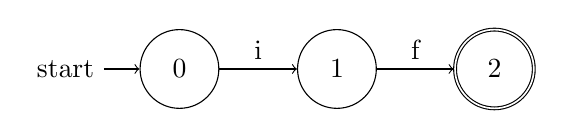
\begin{tikzpicture}
                                \node[state, minimum size=1cm, initial] (0) at (0, 0) {$0$};
                                \node[state, minimum size=1cm] (1) at (2, 0) {$1$};
                                \node[state, minimum size=1cm, accepting] (2) at (4, 0) {$2$};

                                \draw
                                (0) edge[->, above] node{i} (1)
                                (1) edge[->, above] node{f} (2);
                            \end{tikzpicture}
                        \end{center}
                        The example above is deterministic as there are no two transitions from the same state with the same symbol.
                    \item \textbf{non-deterministic finite automata (NFA)}
                        \begin{center}
                            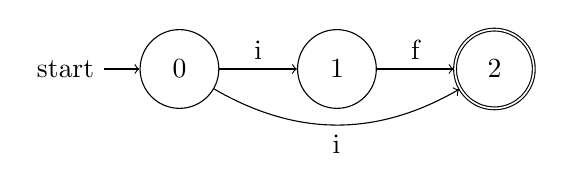
\begin{tikzpicture}
                                \node[state, minimum size=1cm, initial] (0) at (0, 0) {$0$};
                                \node[state, minimum size=1cm] (1) at (2, 0) {$1$};
                                \node[state, minimum size=1cm, accepting] (2) at (4, 0) {$2$};

                                \draw
                                (0) edge[->, above] node{i} (1)
                                (0) edge[->, bend right=30, below] node{i} (2)
                                (1) edge[->, above] node{f} (2);
                            \end{tikzpicture}
                        \end{center}
                        The example above is non-deterministic as there is more than one transition from state 0 with the same symbol.
                        It allows for choice and more compact solutions, but requires backtracking.
                \end{itemize}
            \subsubsection*{Conversion of Regex to (Non-Deterministic) Finite Automata}
                \textbf{Thompson's construction} uses $\epsilon$-transitions to "glue" together automata.
                While this is usually represented with an $\epsilon$ over the transition, it can be omitted for brevity, and therefore any transitions without labels will be assumed to be $\epsilon$-transitions.
                In lieu of repeatedly drawing the same thing, let the regular expression ~R1~ have an initial state of $p$ and an accepting / end state of $q$, and let ~R2~ have an initial state $r$ and accepting state $s$.
                Also note that within the dotted lines can exist an arbitrarily complex automata.
                \begin{center}
                    \begin{tabular}{>{\centering\arraybackslash}m{1.5cm}>{\centering\arraybackslash}m{10cm}}
                        regex & FA \\
                        \hline \\
                        ~a~ &
                        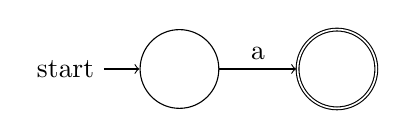
\begin{tikzpicture}
                            \node[state, minimum size=1cm, initial] (0) at (0, 0) {};
                            \node[state, minimum size=1cm, accepting] (1) at (2, 0) {};

                            \draw
                            (0) edge[->, above] node{a} (1);
                        \end{tikzpicture} \\
                        $\epsilon$ &
                        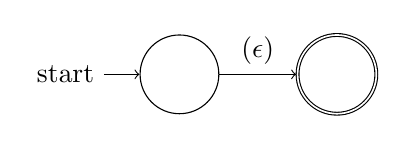
\begin{tikzpicture}
                            \node[state, minimum size=1cm, initial] (0) at (0, 0) {};
                            \node[state, minimum size=1cm, accepting] (1) at (2, 0) {};

                            \draw
                            (0) edge[->, above] node{$(\epsilon)$} (1);
                        \end{tikzpicture} \\
                        ~R1~ &
                        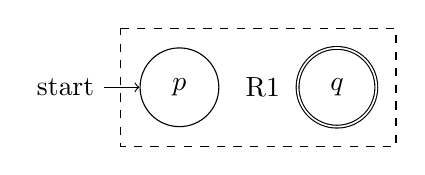
\begin{tikzpicture}
                            \node[state, minimum size=1cm, initial] (p) at (0, 0) {$p$};
                            \node[state, minimum size=1cm, accepting] (q) at (2, 0) {$q$};

                            \node at ($0.5*(p) + 0.5*(q)$) {~R1~};

                            \draw[dashed] ($(p) + (-0.75, 0.75)$) -- ($(q) + (0.75, 0.75)$) -- ($(q) + (0.75, -0.75)$) -- ($(p) + (-0.75, -0.75)$) -- cycle;
                        \end{tikzpicture} \\
                        ~R1 R2~ &
                        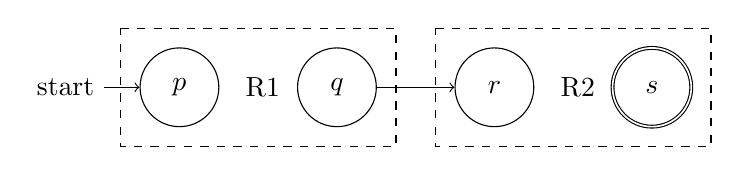
\begin{tikzpicture}
                            \node[state, minimum size=1cm, initial] (p) at (0, 0) {$p$};
                            \node[state, minimum size=1cm] (q) at (2, 0) {$q$};

                            \node at ($0.5*(p) + 0.5*(q)$) {~R1~};

                            \draw[dashed] ($(p) + (-0.75, 0.75)$) -- ($(q) + (0.75, 0.75)$) -- ($(q) + (0.75, -0.75)$) -- ($(p) + (-0.75, -0.75)$) -- cycle;

                            \node[state, minimum size=1cm] (r) at (4, 0) {$r$};
                            \node[state, minimum size=1cm, accepting] (s) at (6, 0) {$s$};

                            \node at ($0.5*(r) + 0.5*(s)$) {~R2~};

                            \draw[dashed] ($(r) + (-0.75, 0.75)$) -- ($(s) + (0.75, 0.75)$) -- ($(s) + (0.75, -0.75)$) -- ($(r) + (-0.75, -0.75)$) -- cycle;

                            \draw (q) edge[->] (r);
                        \end{tikzpicture} \\
                        ~R1|R2~ &
                        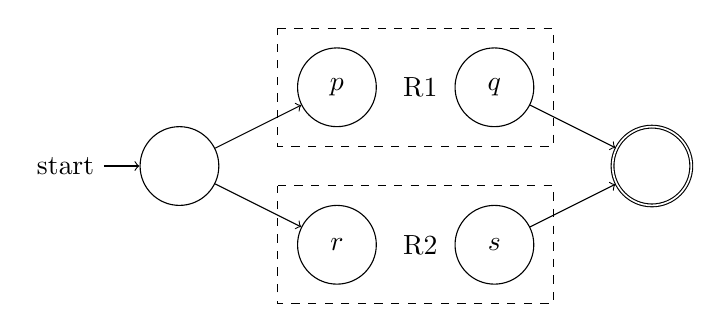
\begin{tikzpicture}
                            \node[state, minimum size=1cm, initial] (0) at (0, 0) {};
                            \node[state, minimum size=1cm, accepting] (1) at (6, 0) {};

                            \node[state, minimum size=1cm] (p) at (2, 1) {$p$};
                            \node[state, minimum size=1cm] (q) at (4, 1) {$q$};

                            \node at ($0.5*(p) + 0.5*(q)$) {~R1~};

                            \draw[dashed] ($(p) + (-0.75, 0.75)$) -- ($(q) + (0.75, 0.75)$) -- ($(q) + (0.75, -0.75)$) -- ($(p) + (-0.75, -0.75)$) -- cycle;

                            \node[state, minimum size=1cm] (r) at (2, -1) {$r$};
                            \node[state, minimum size=1cm] (s) at (4, -1) {$s$};

                            \node at ($0.5*(r) + 0.5*(s)$) {~R2~};

                            \draw[dashed] ($(r) + (-0.75, 0.75)$) -- ($(s) + (0.75, 0.75)$) -- ($(s) + (0.75, -0.75)$) -- ($(r) + (-0.75, -0.75)$) -- cycle;

                            \draw
                            (0) edge[->] (p)
                            (0) edge[->] (r)
                            (q) edge[->] (1)
                            (s) edge[->] (1);
                        \end{tikzpicture} \\
                        ~R1*~ &
                        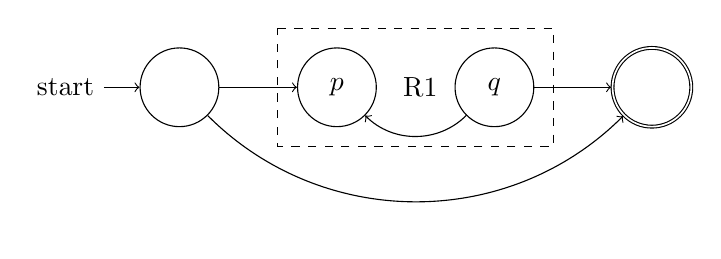
\begin{tikzpicture}
                            \node[state, minimum size=1cm, initial] (0) at (0, 0) {};
                            \node[state, minimum size=1cm, accepting] (1) at (6, 0) {};

                            \node[state, minimum size=1cm] (p) at (2, 0) {$p$};
                            \node[state, minimum size=1cm] (q) at (4, 0) {$q$};

                            \node at ($0.5*(p) + 0.5*(q)$) {~R1~};

                            \draw[dashed] ($(p) + (-0.75, 0.75)$) -- ($(q) + (0.75, 0.75)$) -- ($(q) + (0.75, -0.75)$) -- ($(p) + (-0.75, -0.75)$) -- cycle;

                            \draw
                            (0) edge[->] (p)
                            (0) edge[->, bend right=45] (1)
                            (q) edge[->] (1)
                            (q) edge[->, bend left=45] (p);
                        \end{tikzpicture} \\
                        \hline
                    \end{tabular}
                \end{center}
                For example, consider the regular expressions for an identifier, following the form ~L(L | D)*~, which represents a letter followed by any combination of letters and digits.
                Note that we are allowed to abbreviate the use of ~Letter~ to ~L~, for brevity, and similar for ~Digit~ to ~D~.
                \begin{center}
                    \begin{tikzpicture}
                        \node[state, minimum size=1cm, initial] (0) at (0, 0) {};
                        \node[state, minimum size=1cm] (1) at (2, 0) {};
                        \node[state, minimum size=1cm] (2) at (4, 0) {};
                        \node[state, minimum size=1cm] (3) at (10, 0) {};
                        \node[state, minimum size=1cm, accepting] (4) at (12, 0) {};
                        \node[state, minimum size=1cm] (l1) at (6, 1) {};
                        \node[state, minimum size=1cm] (l2) at (8, 1) {};
                        \node[state, minimum size=1cm] (d1) at (6, -1) {};
                        \node[state, minimum size=1cm] (d2) at (8, -1) {};

                        \draw
                        (0) edge[->, above] node{~L~} (1)
                        (1) edge[->] (2)
                        (1) edge[->, bend right=45] (4)
                        (2) edge[->] (l1)
                        (2) edge[->] (d1)
                        (l1) edge[->, above] node{~L~} (l2)
                        (d1) edge[->, above] node{~D~} (d2)
                        (l2) edge[->] (3)
                        (d2) edge[->] (3)
                        (3) edge[->] (4)
                        (3) edge[->, bend right=75] (2);
                    \end{tikzpicture}
                \end{center}
            \subsubsection*{Conversion from NFA to DFA}
                It's important to note the worst case complexities for NFA and DFA are as follows, where $n$ is the length of the input string, and $r$ is the length of the regular expression;
                \begin{center}
                    \begin{tabular}{l|c|c}
                        type & space complexity & time complexity \\
                        \hline
                        NFA & $O(r)$ & $O(nr)$ \\
                        DFA & $O(2^r)$ & $O(n)$
                    \end{tabular}
                \end{center}
                As you can see, DFAs are much faster, but can be exponentially bigger than NFAs.
                However, the worst case space complexity for a DFA is rarely reached for lexer analyser generators.
                \medskip

                In order to convert from NFA to DFA, we use $\epsilon$-closures.
                To avoid repetition, I will be denoting the $\epsilon$ closure of $s$ as $\epsilon_c(s)$.
                \begin{align*}
                    \epsilon_c(s) & = \text{set of states reachable by zero or more $\epsilon$-transitions from $s$} \\
                    \epsilon_c(\{s_1, \dots, s_n\}) & = \bigcup\limits_{i = 1}^{n} s_i
                \end{align*}
                For example, take the following NFA;
                \begin{center}
                    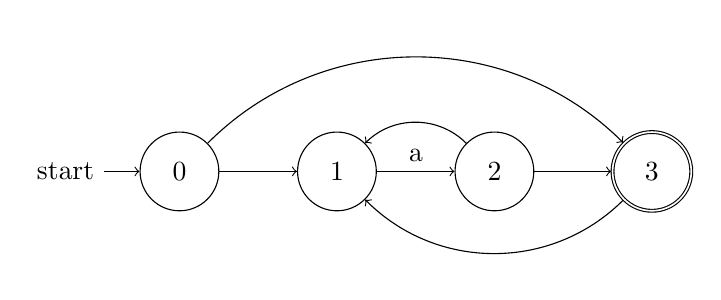
\begin{tikzpicture}
                        \node[state, minimum size=1cm, initial] (0) at (0, 0) {$0$};
                        \node[state, minimum size=1cm] (1) at (2, 0) {$1$};
                        \node[state, minimum size=1cm] (2) at (4, 0) {$2$};
                        \node[state, minimum size=1cm, accepting] (3) at (6, 0) {$3$};

                        \draw
                        (0) edge[->] (1)
                        (0) edge[->, bend left=45] (3)
                        (1) edge[->, above] node{a} (2)
                        (2) edge[->, bend right=45] (1)
                        (2) edge[->] (3)
                        (3) edge[->, bend left=45] (1);
                    \end{tikzpicture}
                \end{center}
                Which has the following closures;
                \begin{align*}
                    \epsilon_c(0) & = \{ 0, 1, 3 \} \\
                    \epsilon_c(1) & = \{ 1 \} \\
                    \epsilon_c(2) & = \{ 1, 2, 3 \} \\
                    \epsilon_c(3) & = \{ 1, 3 \}
                \end{align*}
                From our start state, we then create a node consisting of its $\epsilon$-closure.
                We look at this new node, find the ones that have a non-$\epsilon$-transition, and handle those cases.
                For each new case, we take the state that it goes to, and create a node consisting of its $\epsilon$-closure, and repeat the process.
                Finally, we mark each of the states that contain an accepting state as an accepting state.
                The example above becomes the following;
                \begin{center}
                    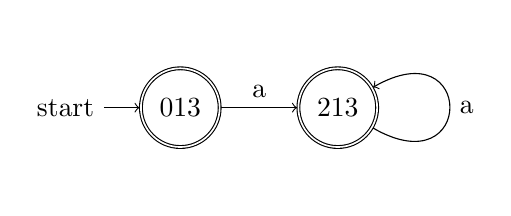
\begin{tikzpicture}
                        \node[state, minimum size=1cm, initial, accepting] (0) at (0, 0) {$013$};
                        \node[state, minimum size=1cm, accepting] (1) at (2, 0) {$213$};
                        \draw
                        (0) edge[->, above] node{a} (1)
                        (1) edge[->, loop, out=-30, in=30, right, distance=1.5cm] node{a} (1);
                    \end{tikzpicture}
                \end{center}
        \subsection*{17th January 2020}
            sss33
\end{document}
